\subsection{Preselection}
\label{sec:eejjPreselection}

A sample of events enriched in SM background processes is 
selected to verify the background estimate in the \eejj~channel.
This \eejj~preselection proceeds with the following cuts
(all the reconstructed objects are required to pass the selection criteria 
described in Chapter~\ref{ch:analysis-object-selection}):
\begin{itemize}
\item Pass the event filters listed in Section \ref{sec:event-filters}
\item Pass the signal triggers listed in Table \ref{tab:eejjDoublePhotEleHLT} (not required for background estimates)
\item Exactly 2 HEEP electrons with $\pt > 40$~\GeV
\item At least 2 jets with $\pt >30$~\GeV and $|\eta|<2.4$
\item No selected muons passing the ID described in Section \ref{sec:id-muon}
\item $\mee > 60$~\GeV
\item $\st>250$~\GeV
\end{itemize}

The $\pt$ cut on the electrons is chosen to be high
enough for the triggers listed in Table \ref{tab:eejjDoublePhotEleHLT}
to be fully efficient.  
The $|\eta|$ cut on the jets rejects potential fake jets reconstructed from anomalous
signals in the HF (which covers the range $|\eta| > 3.0$).  
This cut has a negligable impact on the leptoquark signal efficiency.
The muon veto rejects backgrounds from \ttbar~events with an $e\mu jj$ final state.
The \mee~cut is chosen to be compatible 
with the background MC, which only models $\mee > 50$ GeV.
Both the \mee~and \st~cuts are looser than the cuts applied in the final selection of the \eejj~channel.

At this stage of the selection, there is sufficient data to compare with the background 
predictions for all the observables employed in the final event selection. 
The distribution of the number of reconstructed primary vertices is shown in Figure~\ref{fig:eejj_preselection_vertices}.
The \pt~and $\eta$ distributions of the two leading electrons and the two leading jets are shown in Figures 
\ref{fig:eejj_preselection_ele1}, 
\ref{fig:eejj_preselection_ele2},
\ref{fig:eejj_preselection_jet1}, and 
\ref{fig:eejj_preselection_jet2}. 
The \mee~distribution is shown in Figure~\ref{fig:eejj_preselection_mee}. 
The \st~and \mej~distributions are shown in Figure~\ref{fig:eejj_preselection_st_and_mej}. 

Overall, a good agreement is observed at \eejj~preselection between data and 
background predictions for the shapes of all the distributions of observables employed in the final, 
optimized event selection. An exception is represented by \mee~shape, shown in Figure~\ref{fig:eejj_preselection_mee}, 
for which a discrepancy is visible around the \PZz~mass peak. The data is shifted towards lower 
values of \mee~compared to the simulation, and the distribution of data is wider. This is due to the 
non-optimal ECAL calibration constants used in the reconstruction of data 
(the datasets used in this analysis are listed in Section~\ref{sec:data-samples}).
The discrepancy is more pronounced around the \PZz~mass peak 
compared to the \mee~tails due to the sharpness of the invariant mass shape in that region, 
which amplifies any small discrepancy between data and simulation. This effect 
has a small impact on the final results and it is taken into account in the analysis as a systematic 
uncertainty on the electron energy scale and resolution, as described in detail 
in Chapter~\ref{ch:analysis-systematics}.

\begin{figure*}
  \begin{center}
    {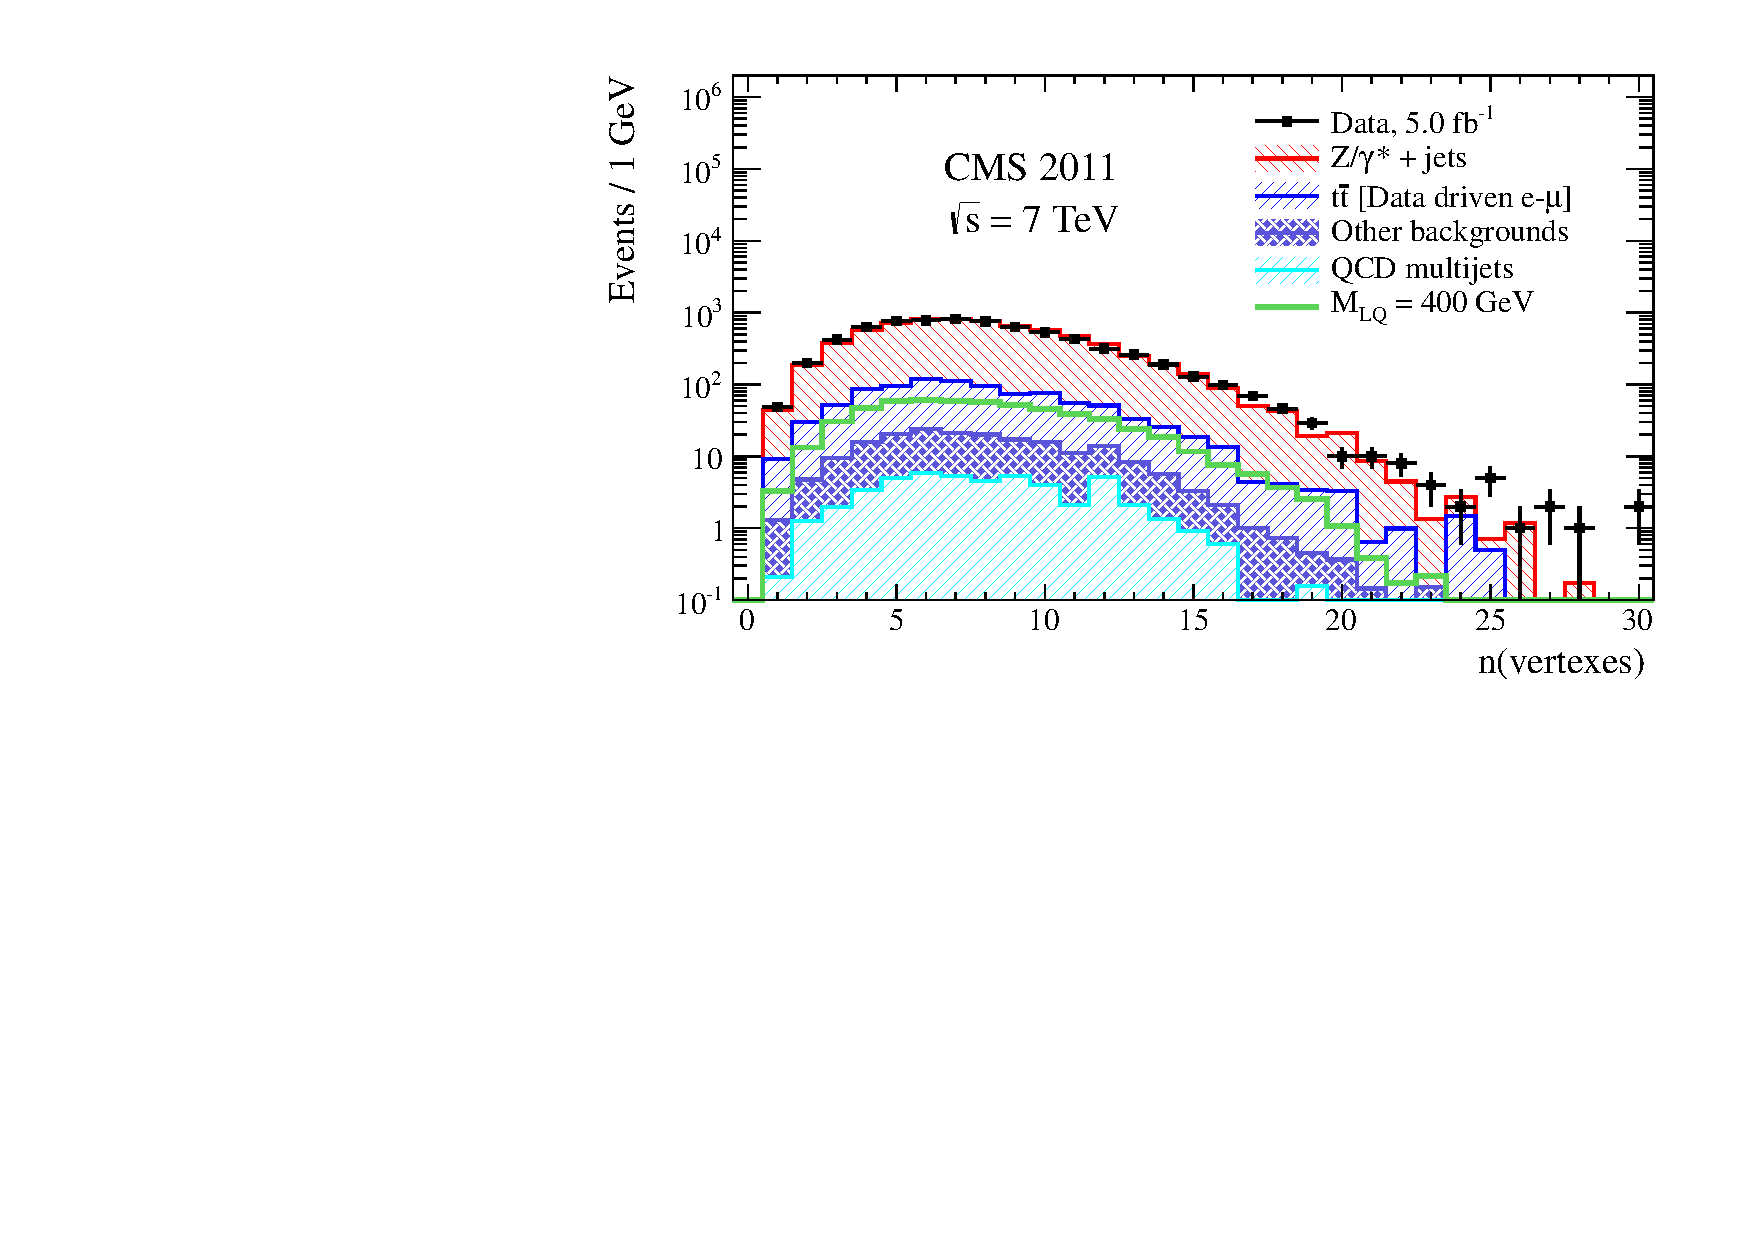
\includegraphics[width=.49\textwidth]{tex/analysis/event_selection/fig/ee/preselection/nVertex_PAS_eejj_WZSherpa_noNSigma.pdf}}\\
    \caption{
      The distribution of the number of primary vertices for events passing the
      \eejj~preselection.
    }
    \label{fig:eejj_preselection_vertices}
  \end{center}
\end{figure*}

\begin{figure*}
  \begin{center}
    {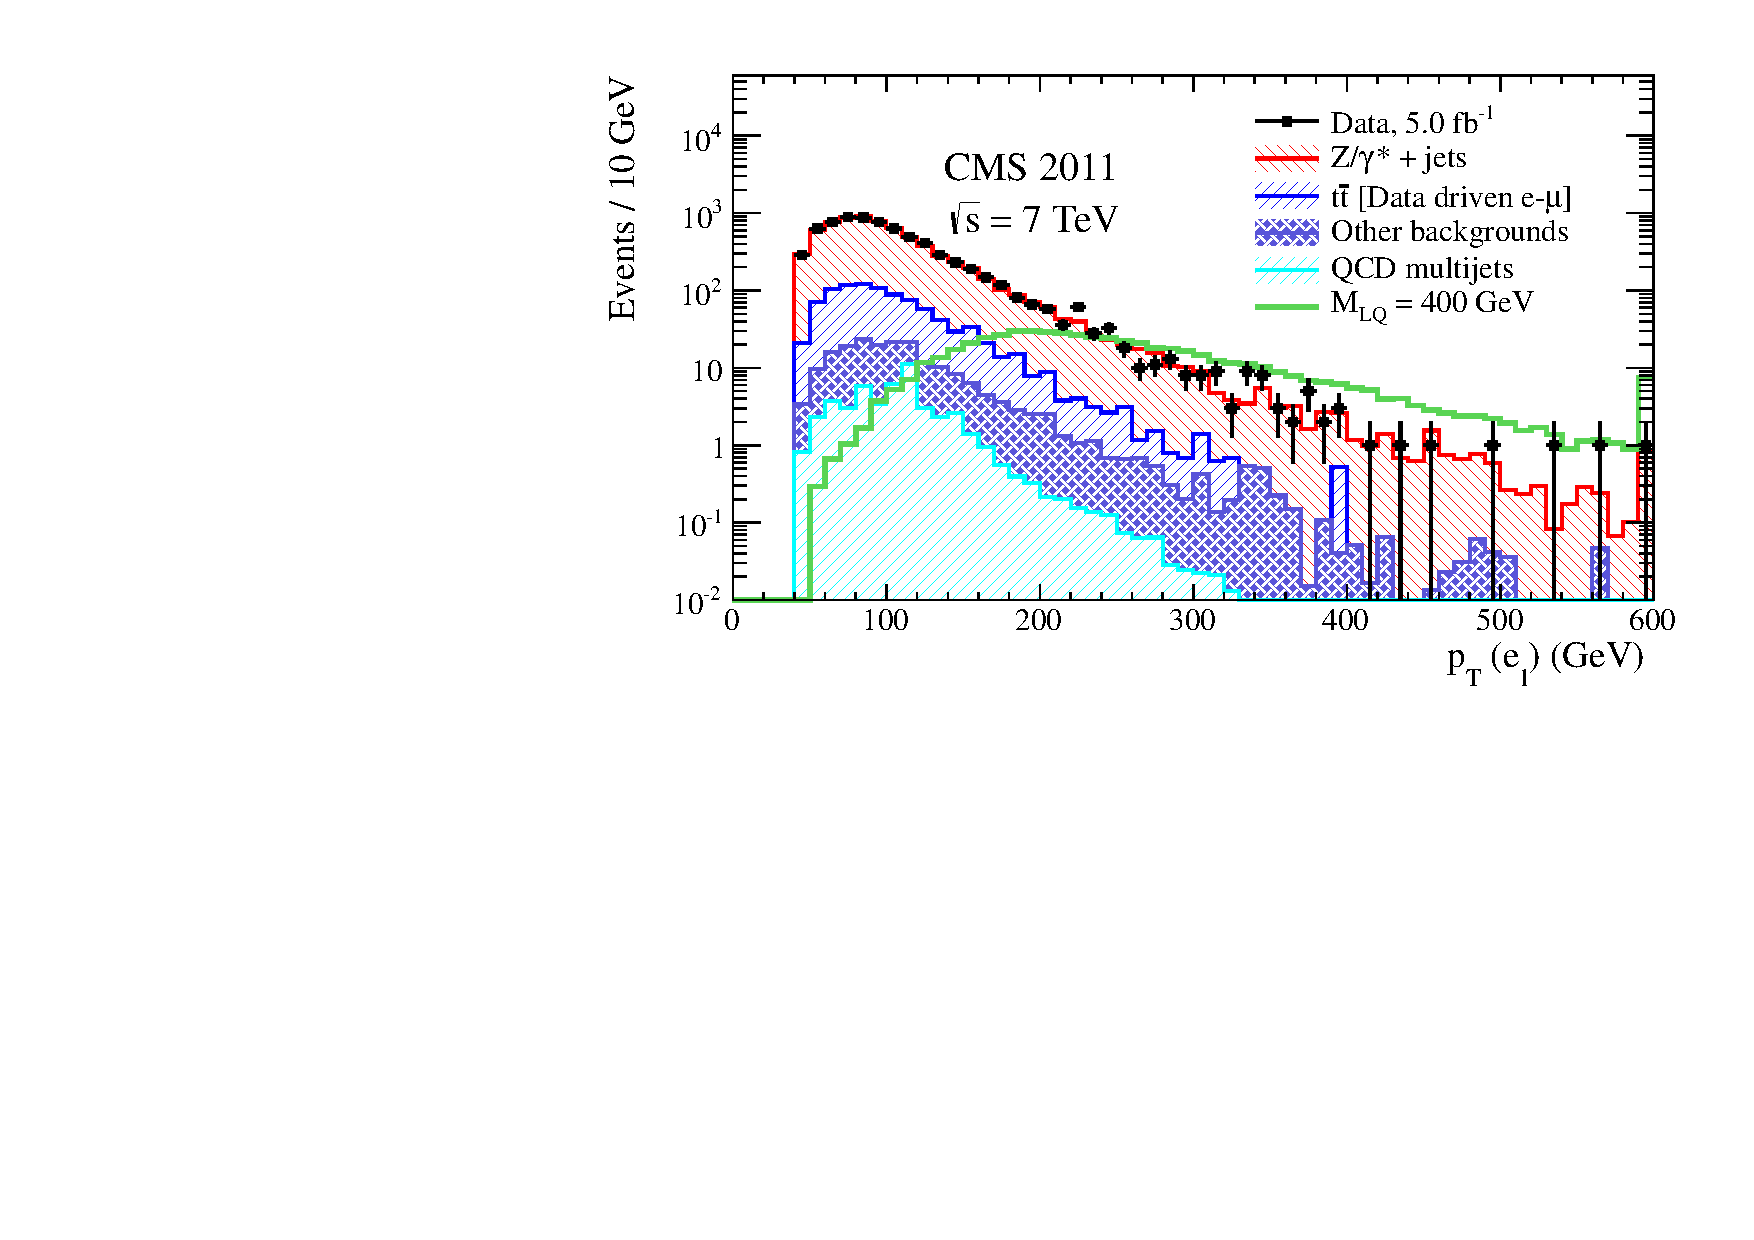
\includegraphics[width=.49\textwidth]{tex/analysis/event_selection/fig/ee/preselection/Pt1stEle_PAS_eejj_WZSherpa_noNSigma.pdf}}
    {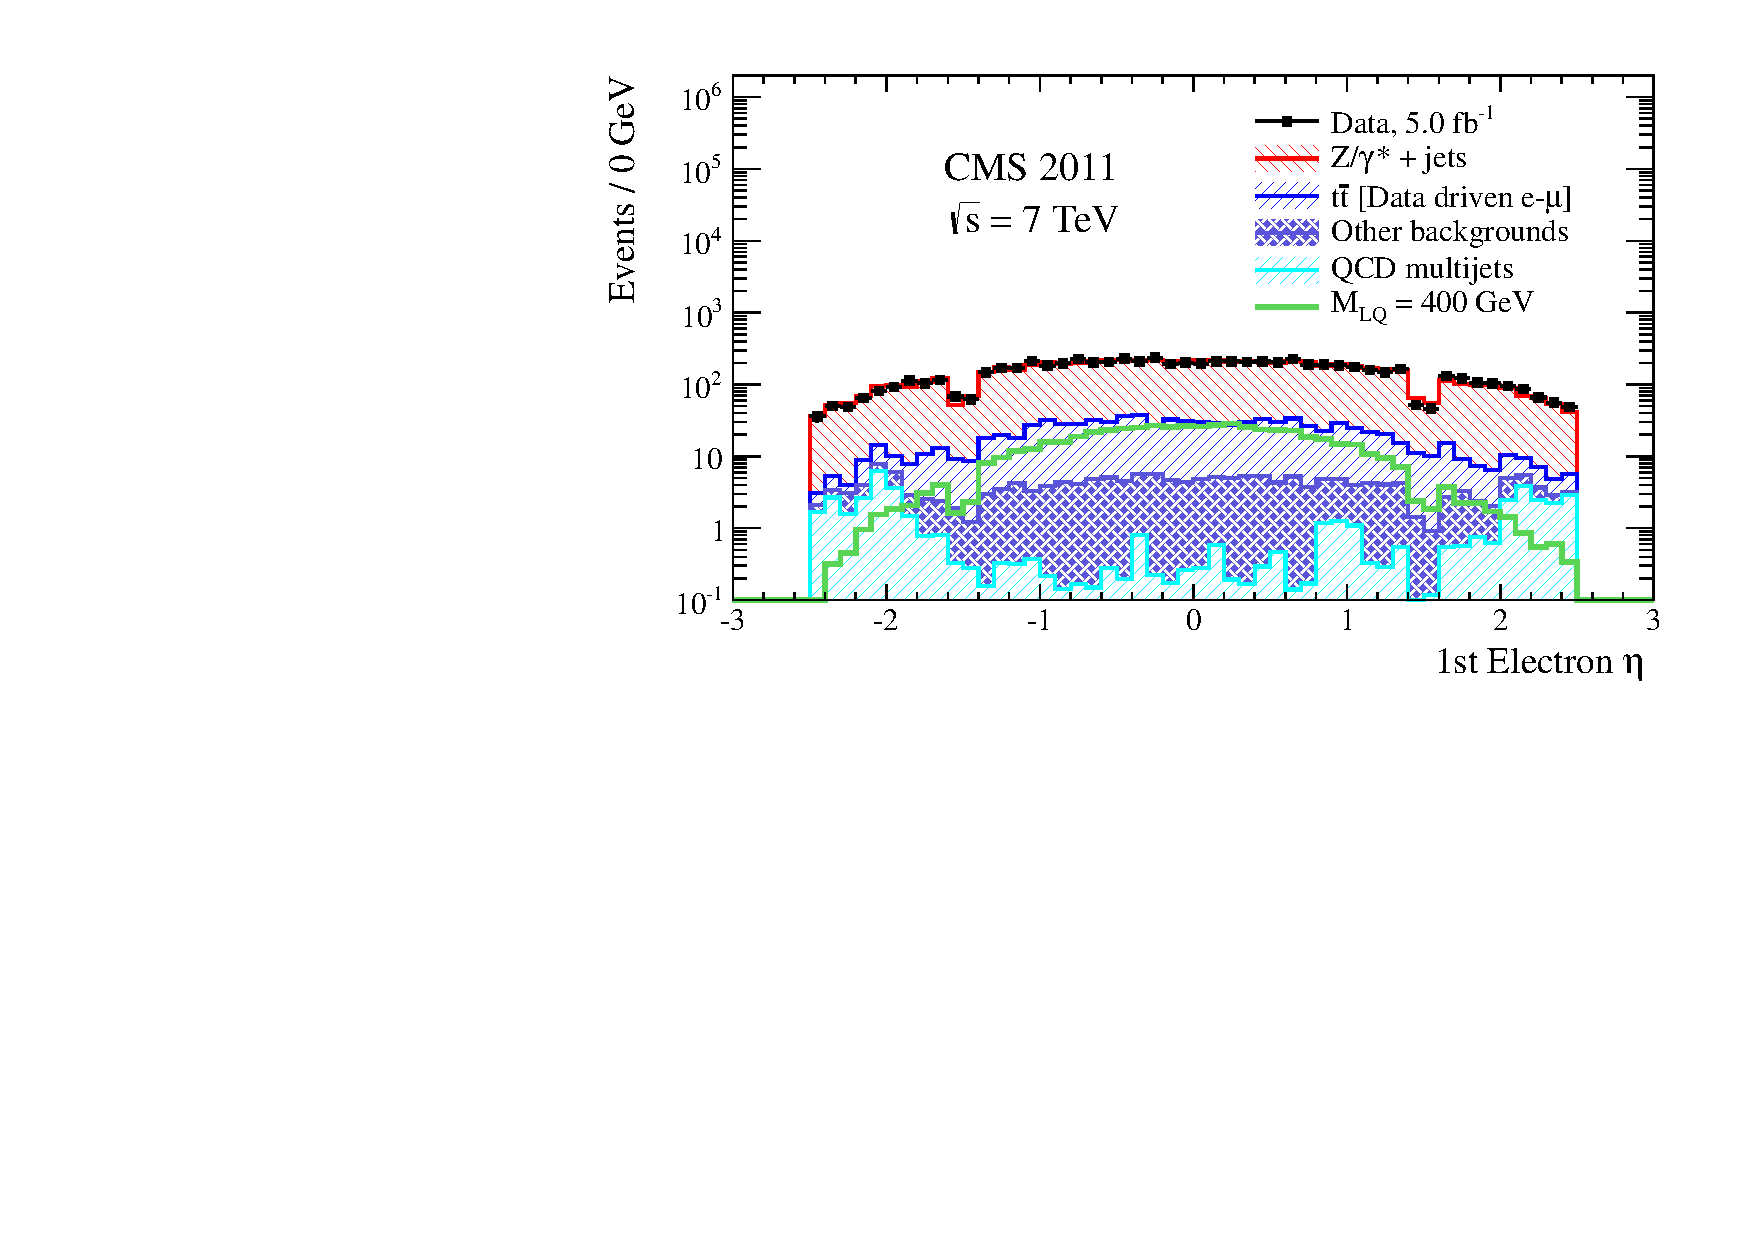
\includegraphics[width=.49\textwidth]{tex/analysis/event_selection/fig/ee/preselection/Eta1stEle_PAS_eejj_WZSherpa_noNSigma.pdf}}
    \caption{
      The \pt~(left) and $\eta$~(right) distributions of the leading
      (in \pt) electron for events passing the \eejj~preselection.
    }
    \label{fig:eejj_preselection_ele1}
  \end{center}
\end{figure*}
\begin{figure*}
  \begin{center}
    {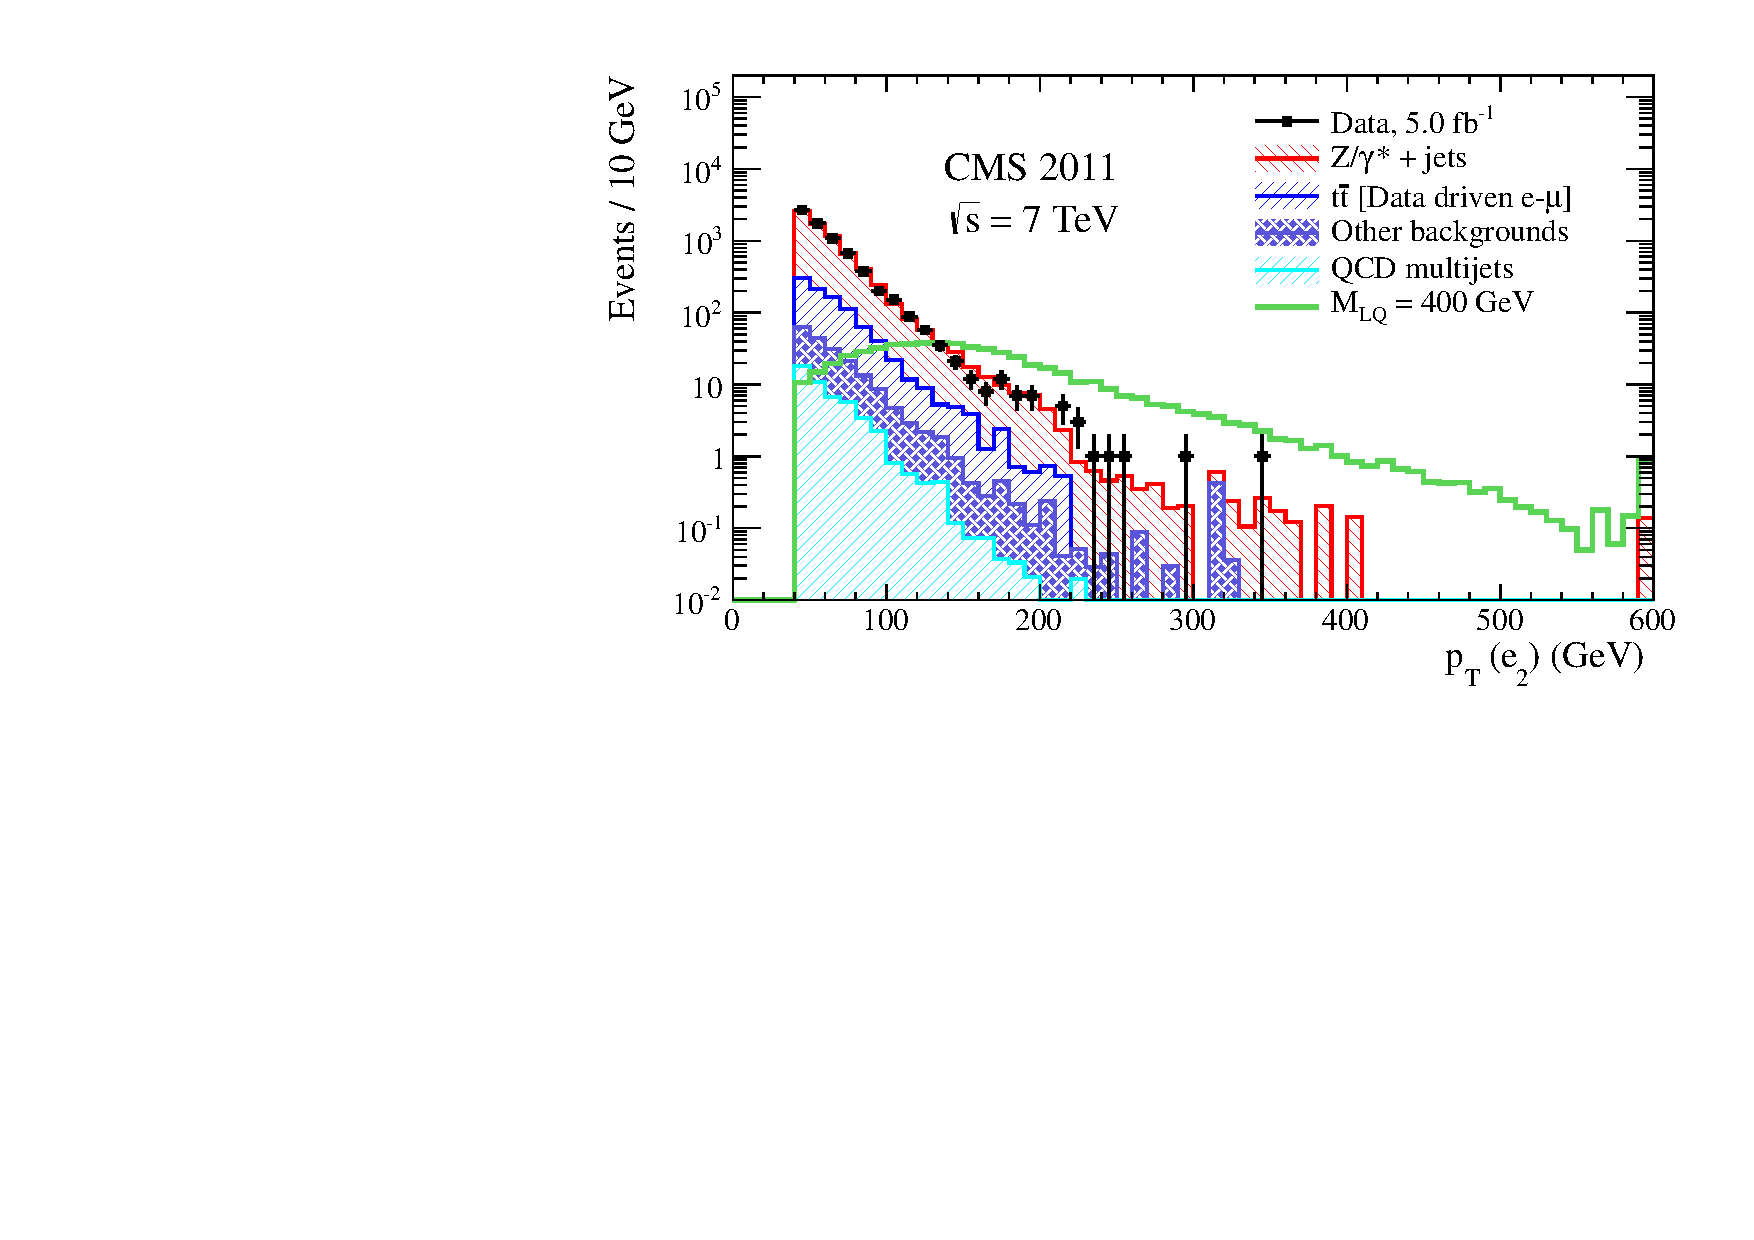
\includegraphics[width=.49\textwidth]{tex/analysis/event_selection/fig/ee/preselection/Pt2ndEle_PAS_eejj_WZSherpa_noNSigma.pdf}}
    {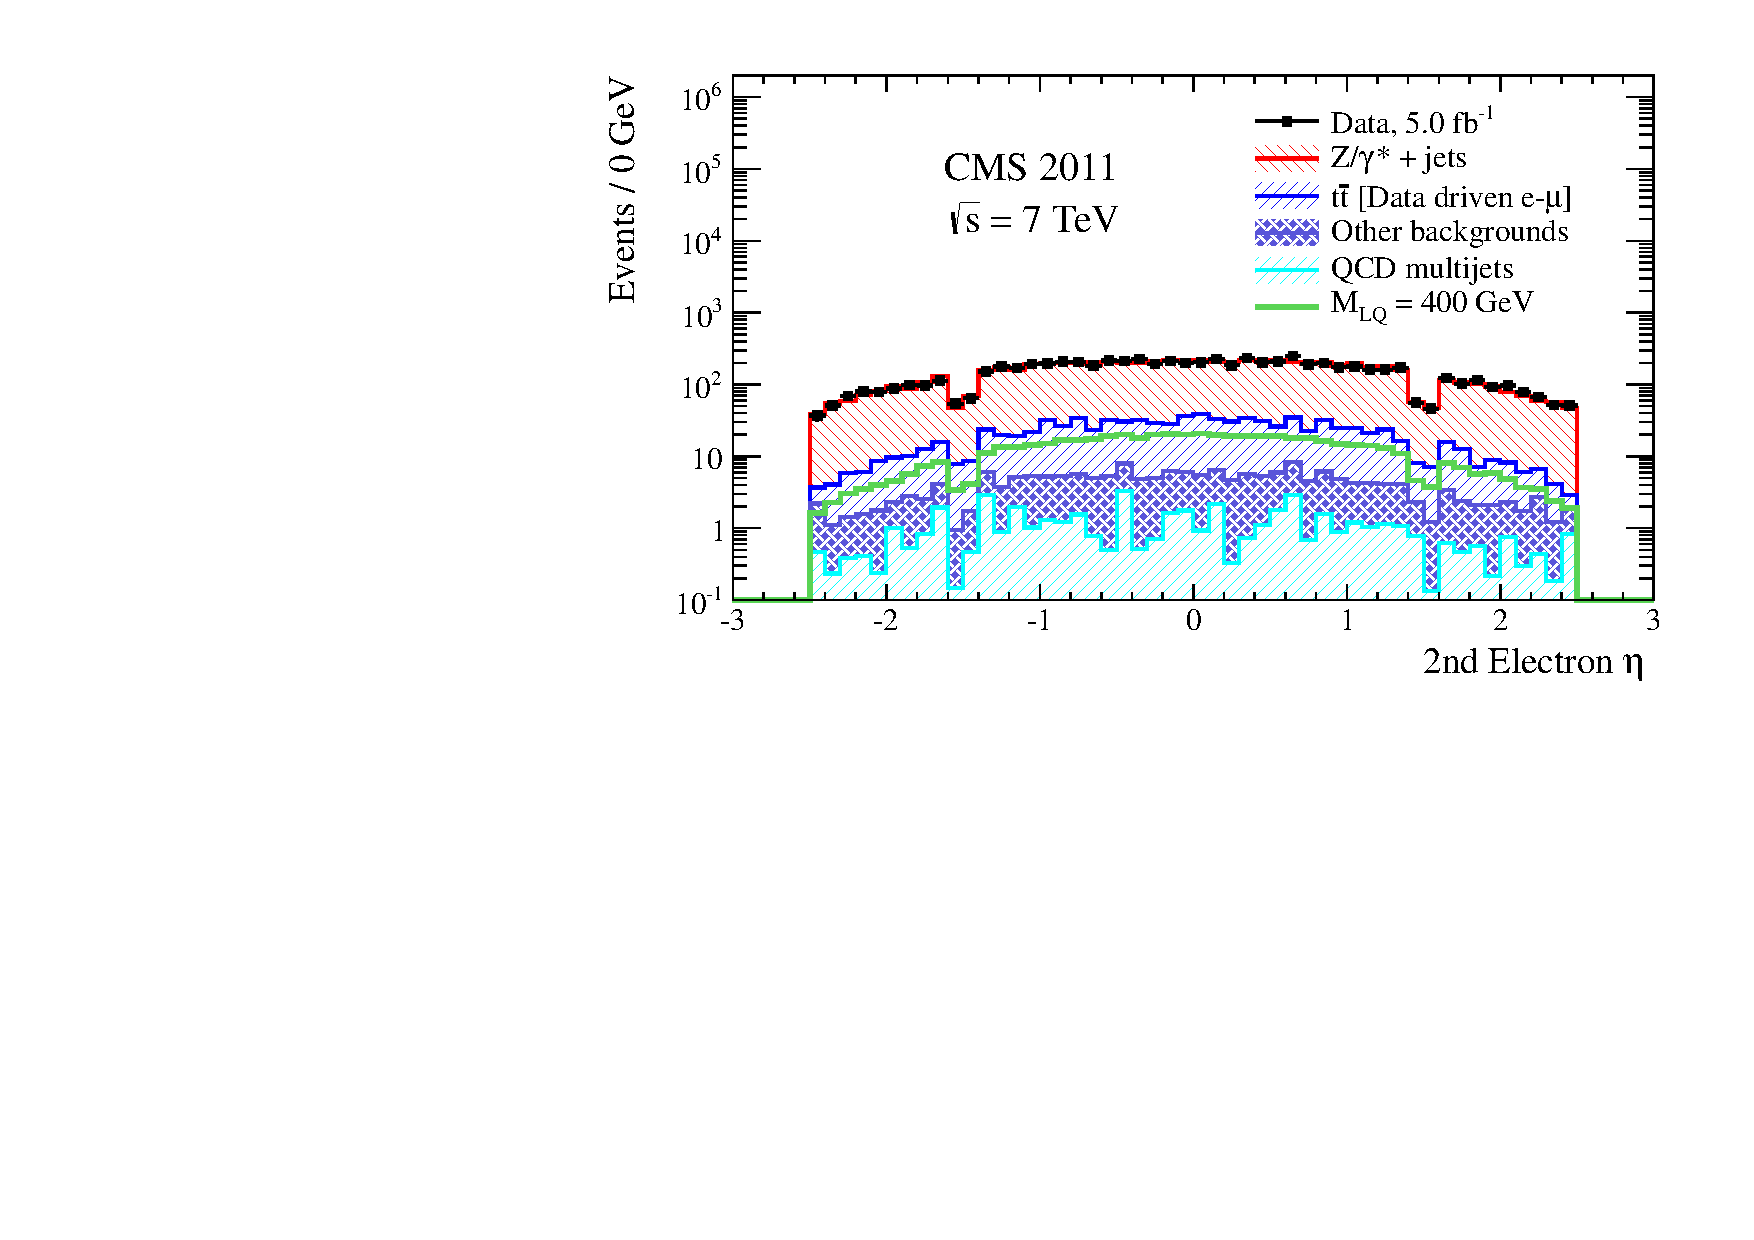
\includegraphics[width=.49\textwidth]{tex/analysis/event_selection/fig/ee/preselection/Eta2ndEle_PAS_eejj_WZSherpa_noNSigma.pdf}}
    \caption{
      The \pt~(left) and $\eta$~(right) distributions of the second leading
      (in \pt) electron for events passing the \eejj~preselection.
    }
    \label{fig:eejj_preselection_ele2}
  \end{center}
\end{figure*}

\begin{figure*}
  \begin{center}
    {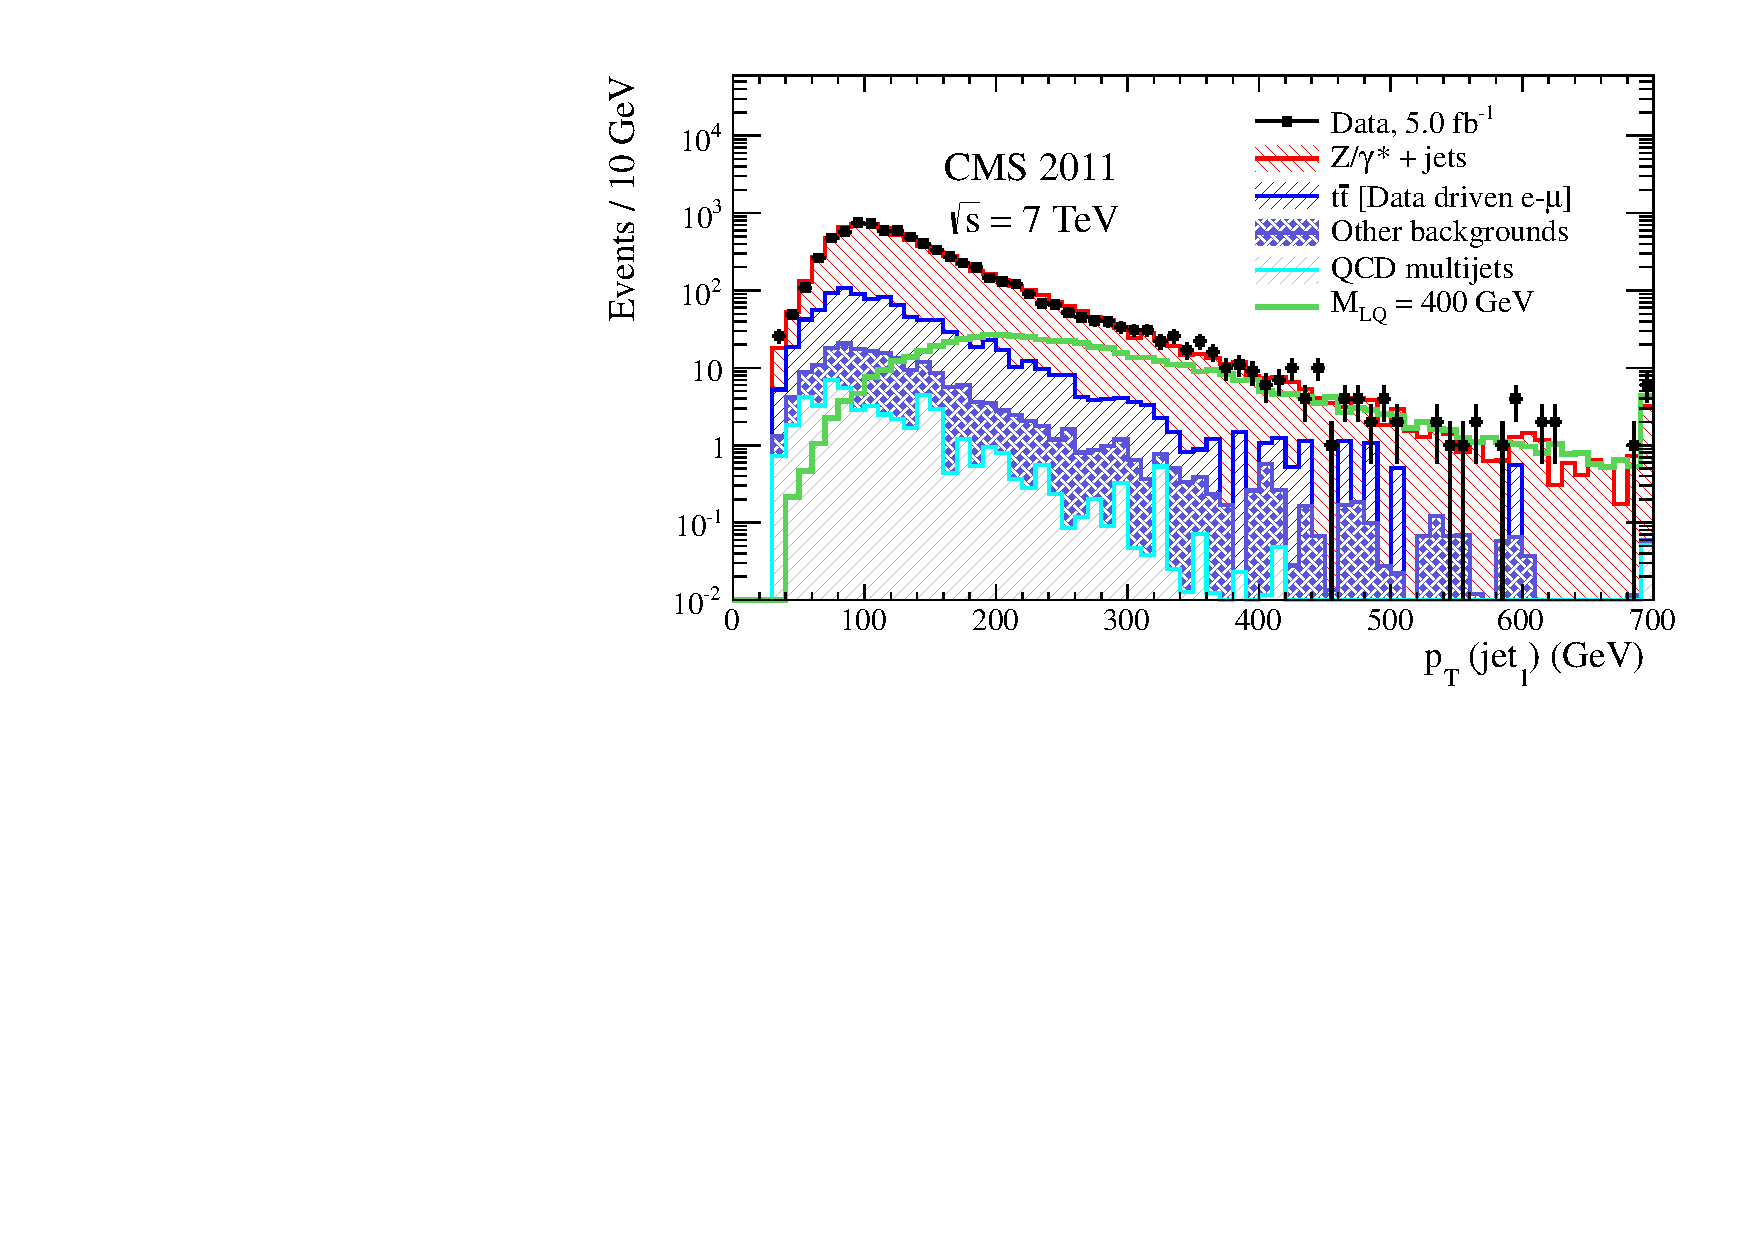
\includegraphics[width=.49\textwidth]{tex/analysis/event_selection/fig/ee/preselection/Pt1stJet_PAS_eejj_WZSherpa_noNSigma.pdf}}
    {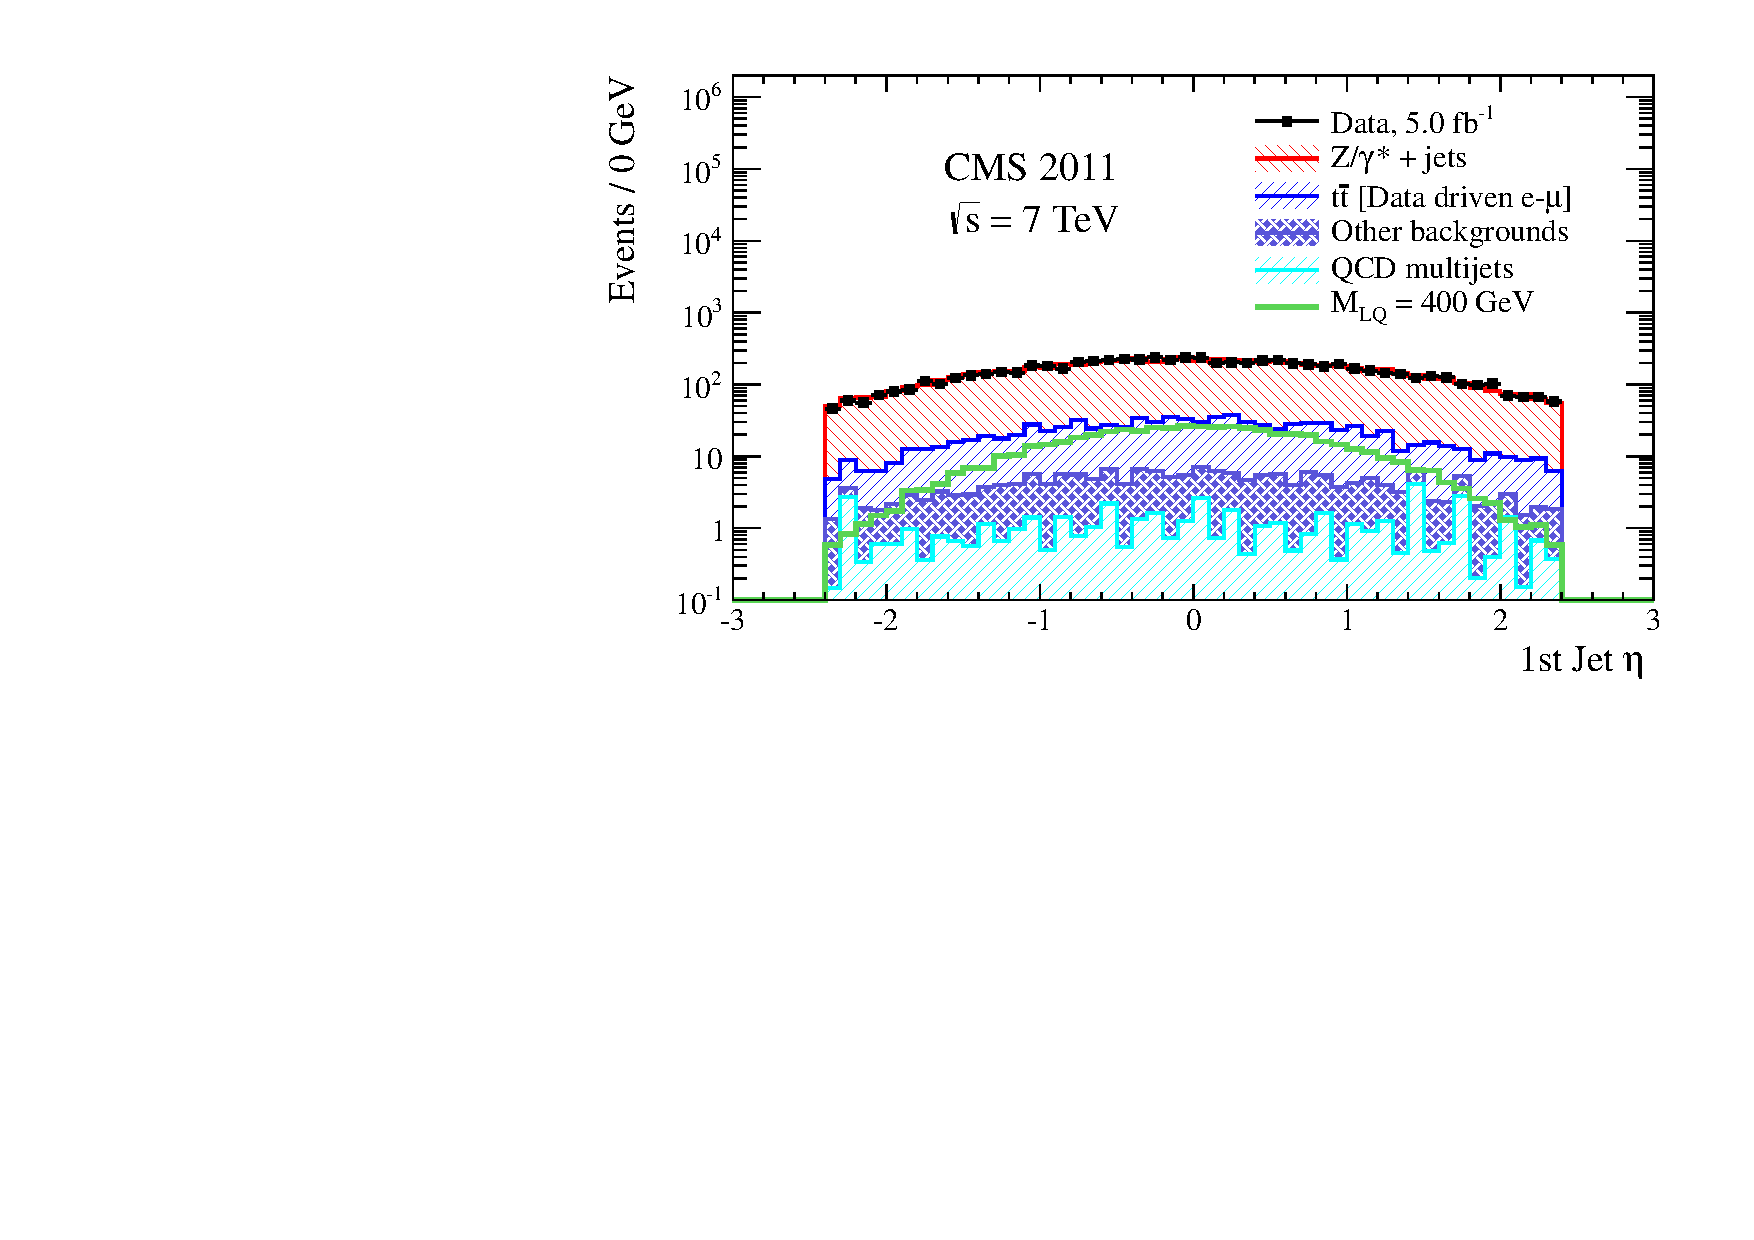
\includegraphics[width=.49\textwidth]{tex/analysis/event_selection/fig/ee/preselection/Eta1stJet_PAS_eejj_WZSherpa_noNSigma.pdf}}
    \caption{
      The \pt~(left) and $\eta$~(right) distributions of the leading
      (in \pt) jet for events passing the \eejj~preselection.
    }
    \label{fig:eejj_preselection_jet1}
  \end{center}
\end{figure*}

\begin{figure*}
  \begin{center}
    {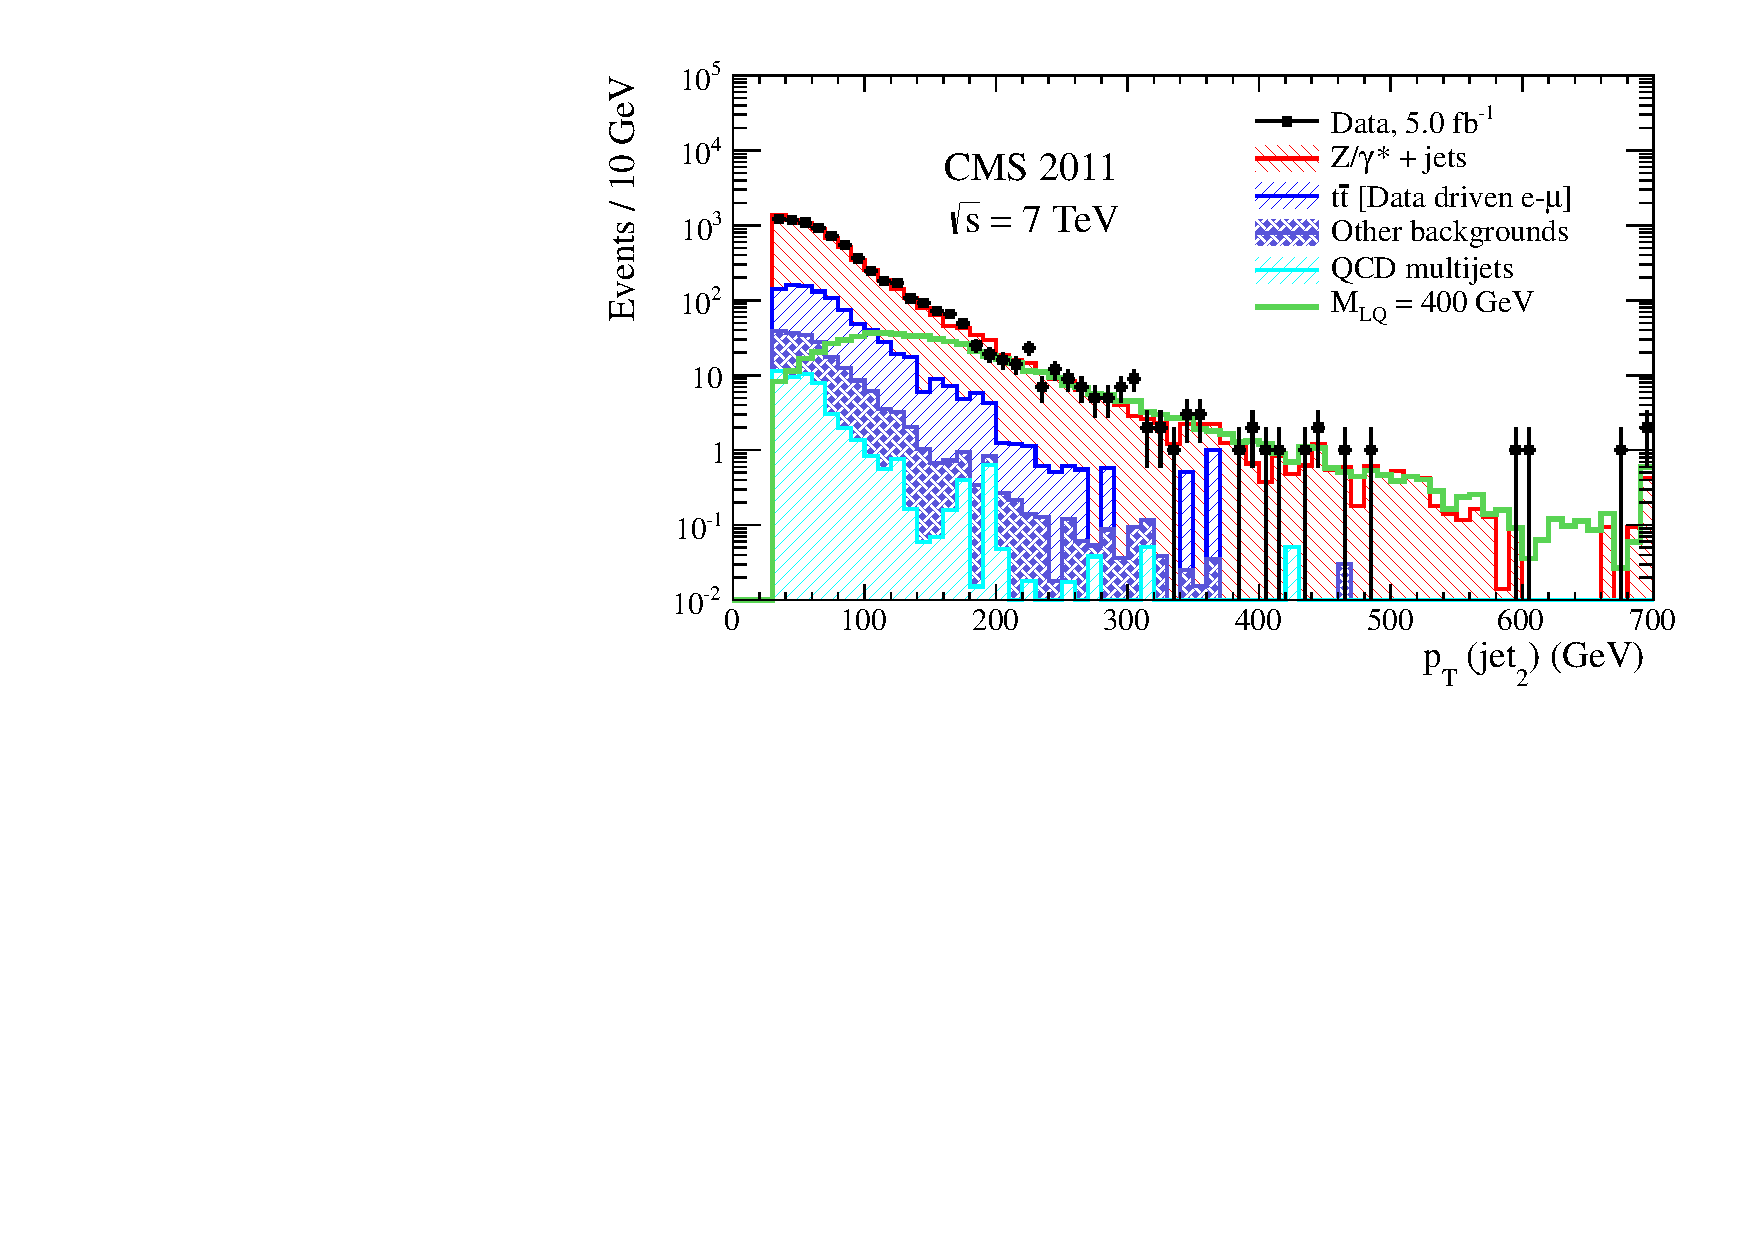
\includegraphics[width=.49\textwidth]{tex/analysis/event_selection/fig/ee/preselection/Pt2ndJet_PAS_eejj_WZSherpa_noNSigma.pdf}}
    {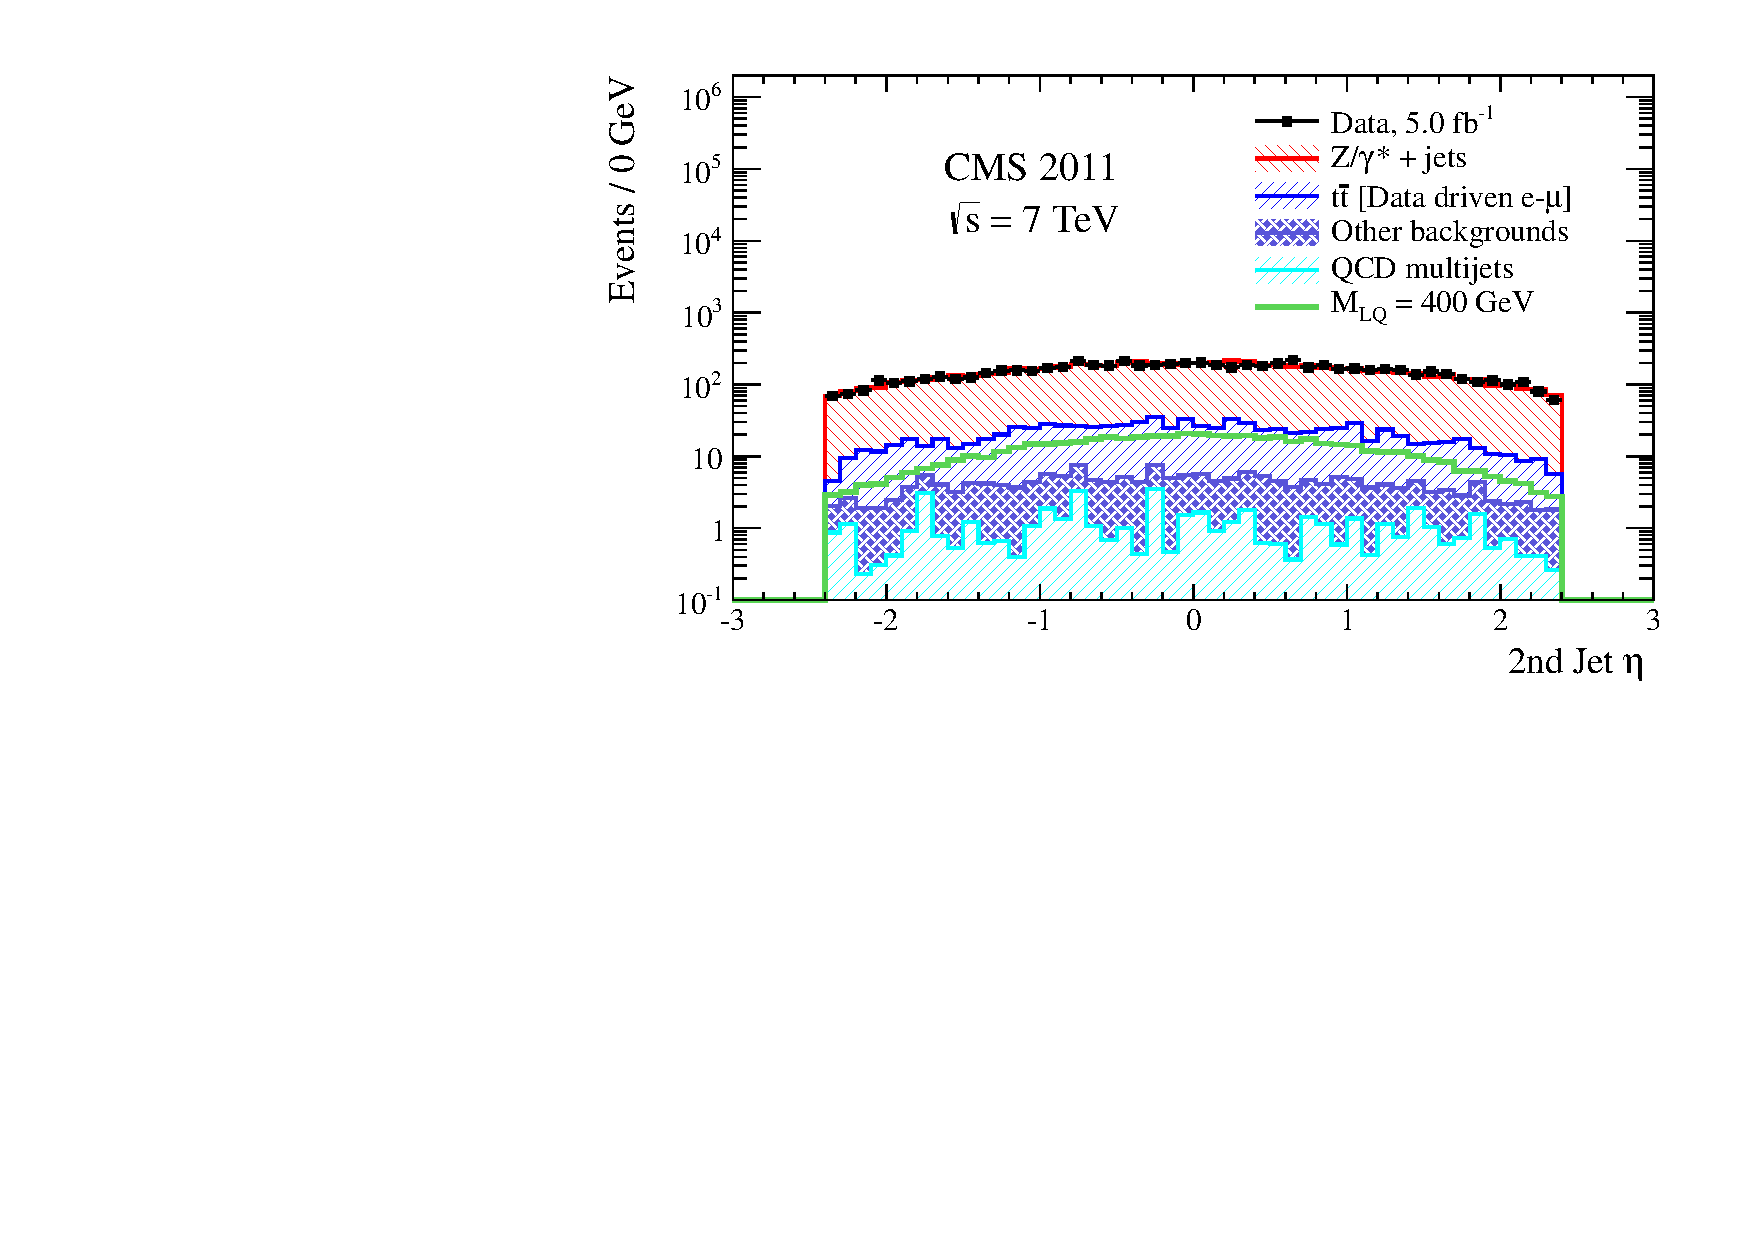
\includegraphics[width=.49\textwidth]{tex/analysis/event_selection/fig/ee/preselection/Eta2ndJet_PAS_eejj_WZSherpa_noNSigma.pdf}}
    \caption{
      The \pt~(left) and $\eta$~(right) distributions of the second leading
      (in \pt) jet for events passing the \eejj~preselection.
    }
    \label{fig:eejj_preselection_jet2}
  \end{center}
\end{figure*}

\begin{figure*}
  \begin{center}
    {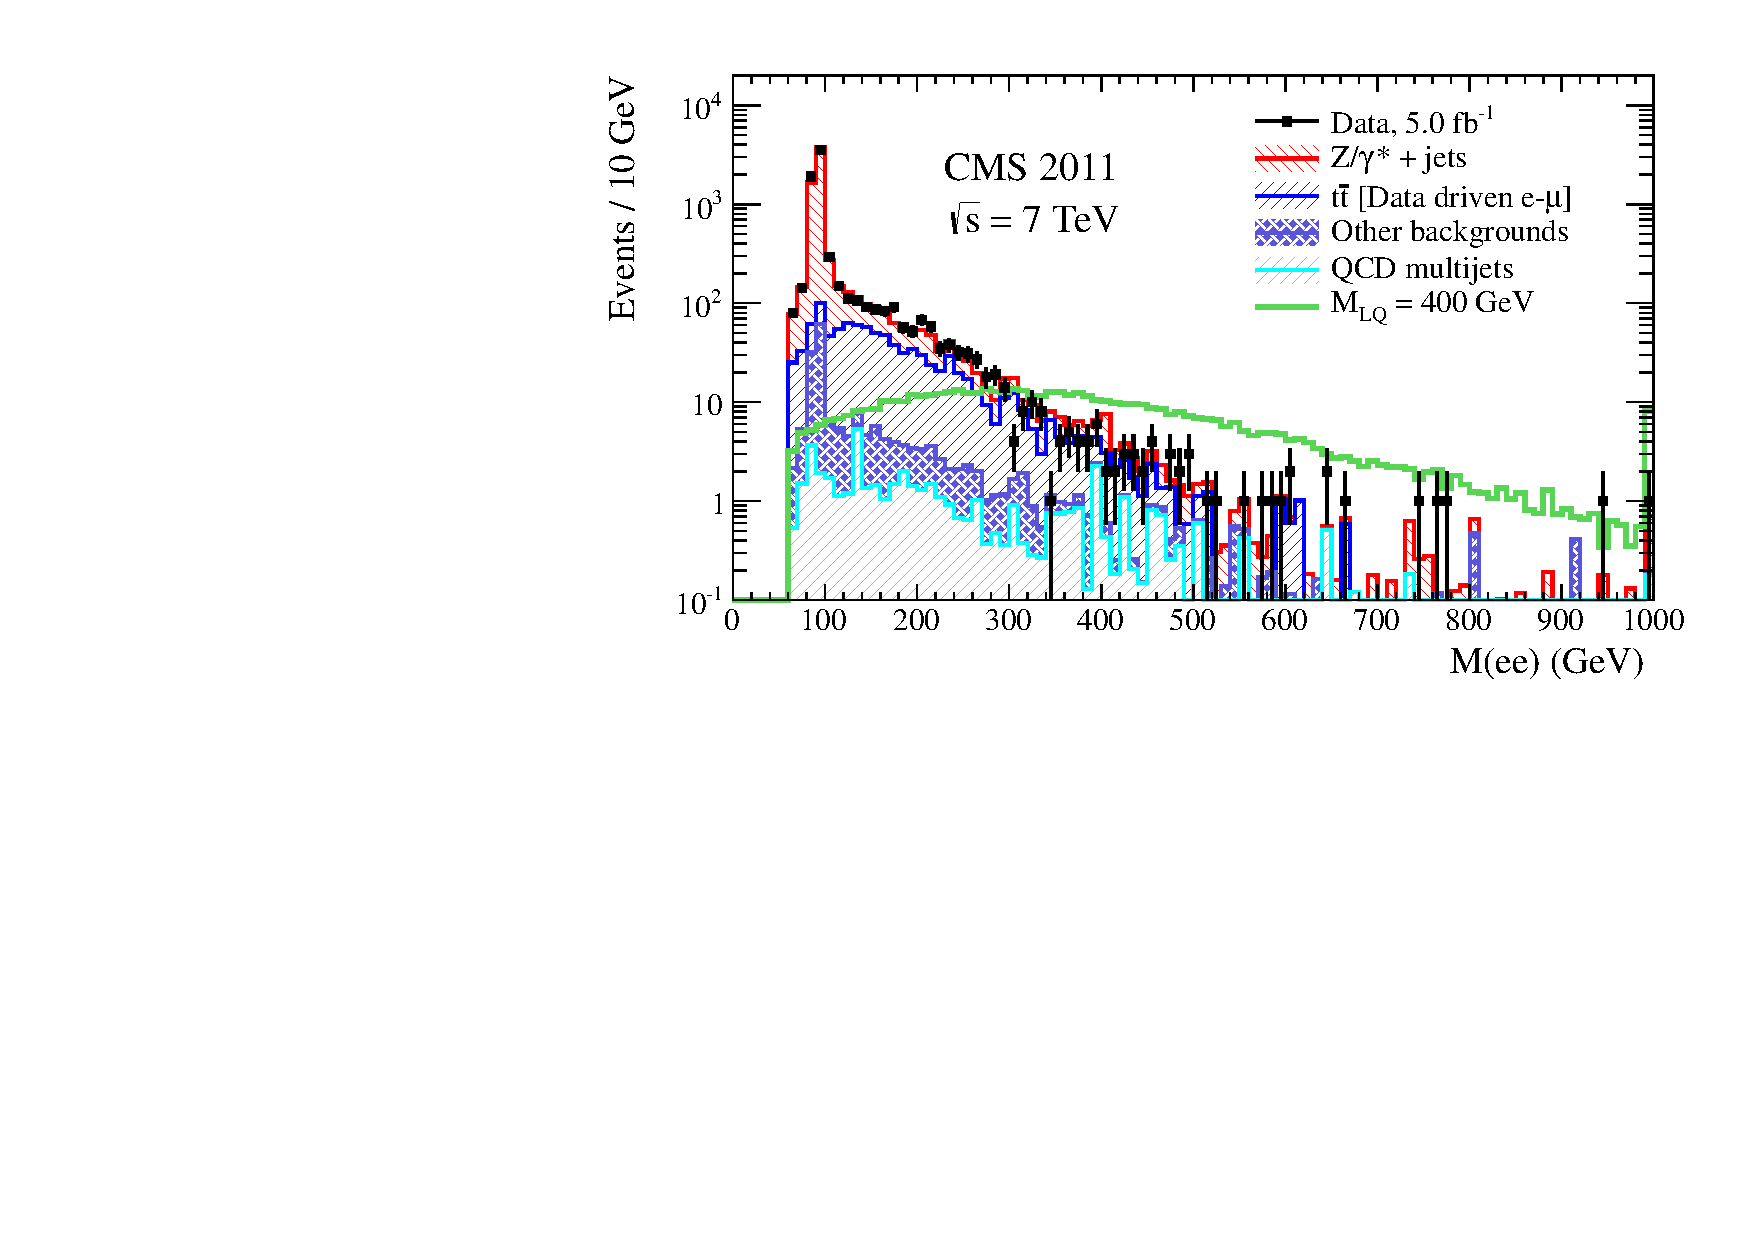
\includegraphics[width=.49\textwidth]{tex/analysis/event_selection/fig/ee/preselection/Mee_PAS_eejj_WZSherpa_noNSigma.pdf}}
    {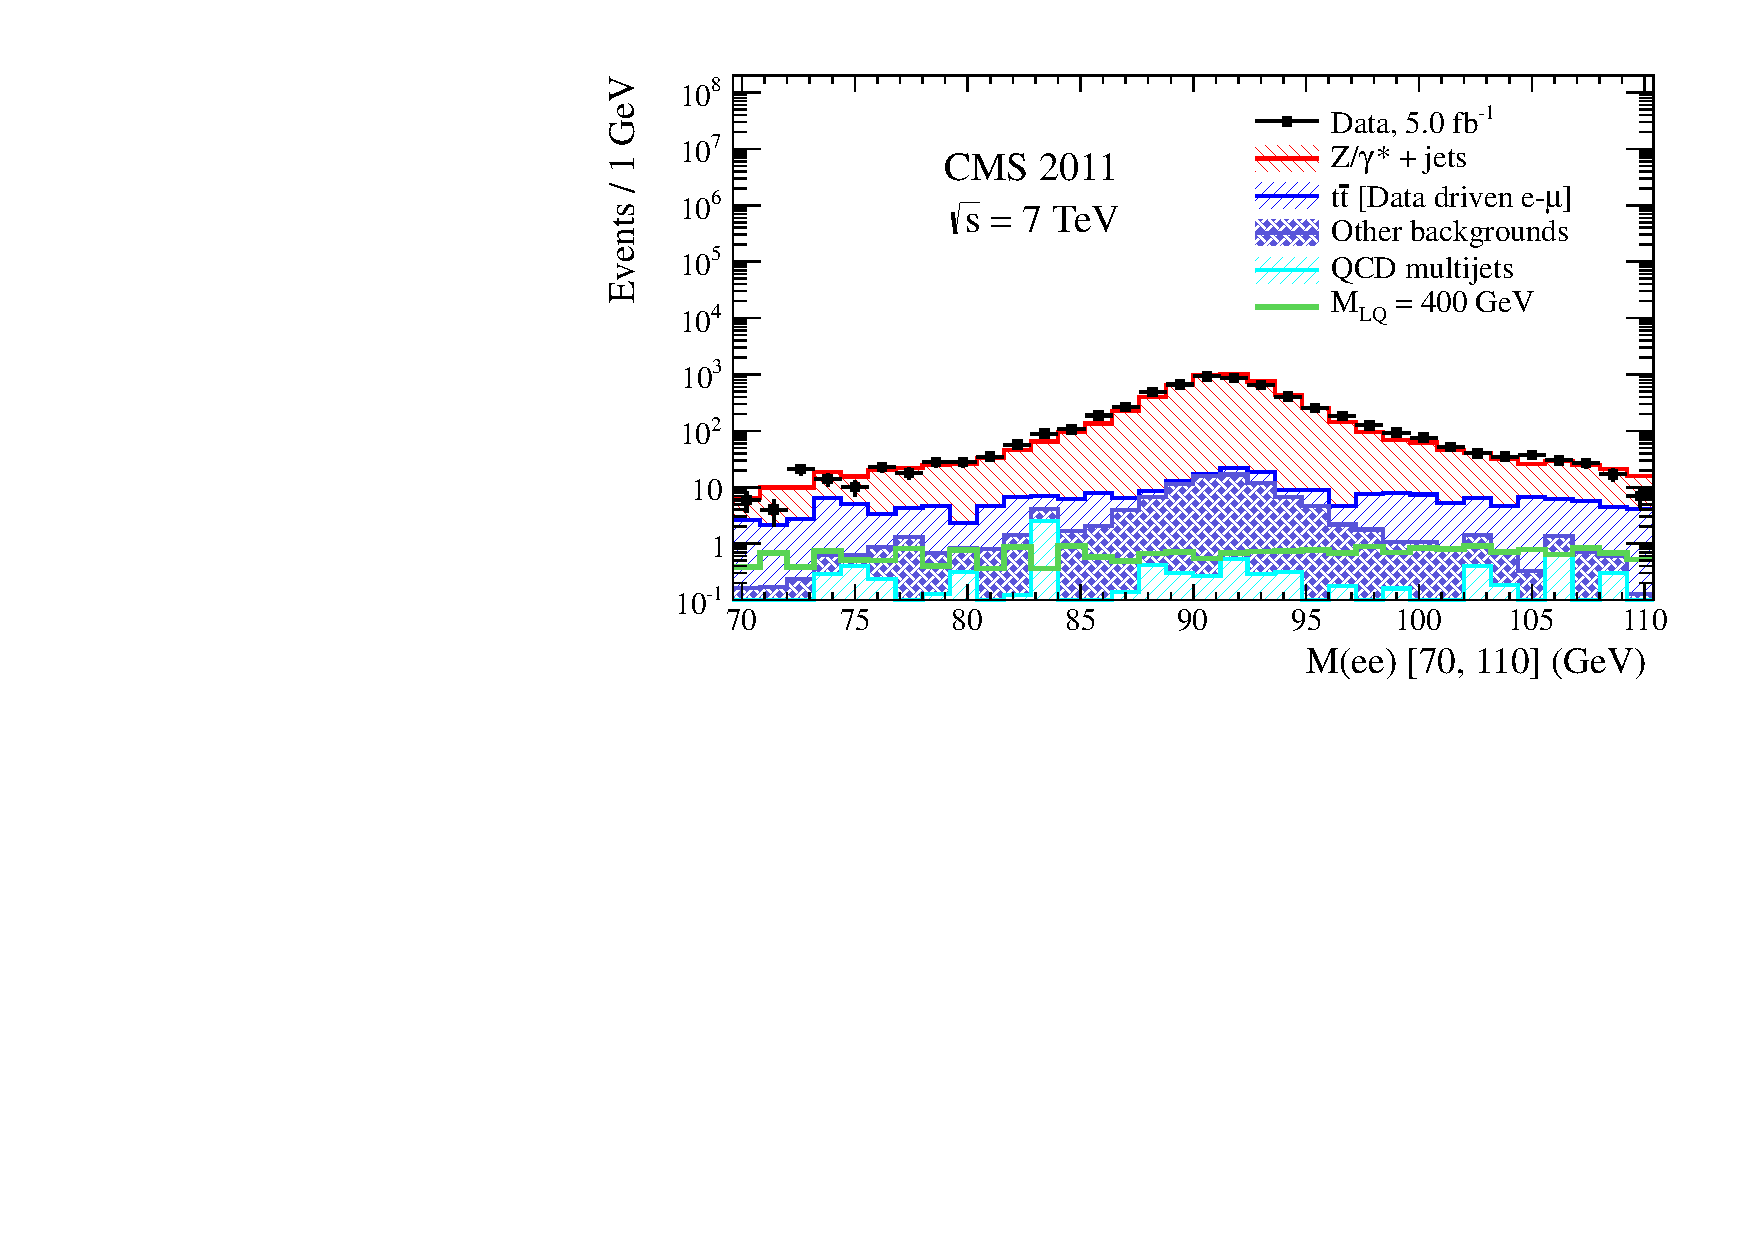
\includegraphics[width=.49\textwidth]{tex/analysis/event_selection/fig/ee/preselection/Mee_70_110_Preselection_eejj_WZSherpa_noNSigma.pdf}}
    \caption{
      The \mee~distribution in the full range (left) and in a zoomed region
      around the $\text{Z}^{0}$ mass peak (right) passing the \eejj~preselection.
    }
    \label{fig:eejj_preselection_mee}
  \end{center}
\end{figure*}

\begin{figure*}
  \begin{center}
    {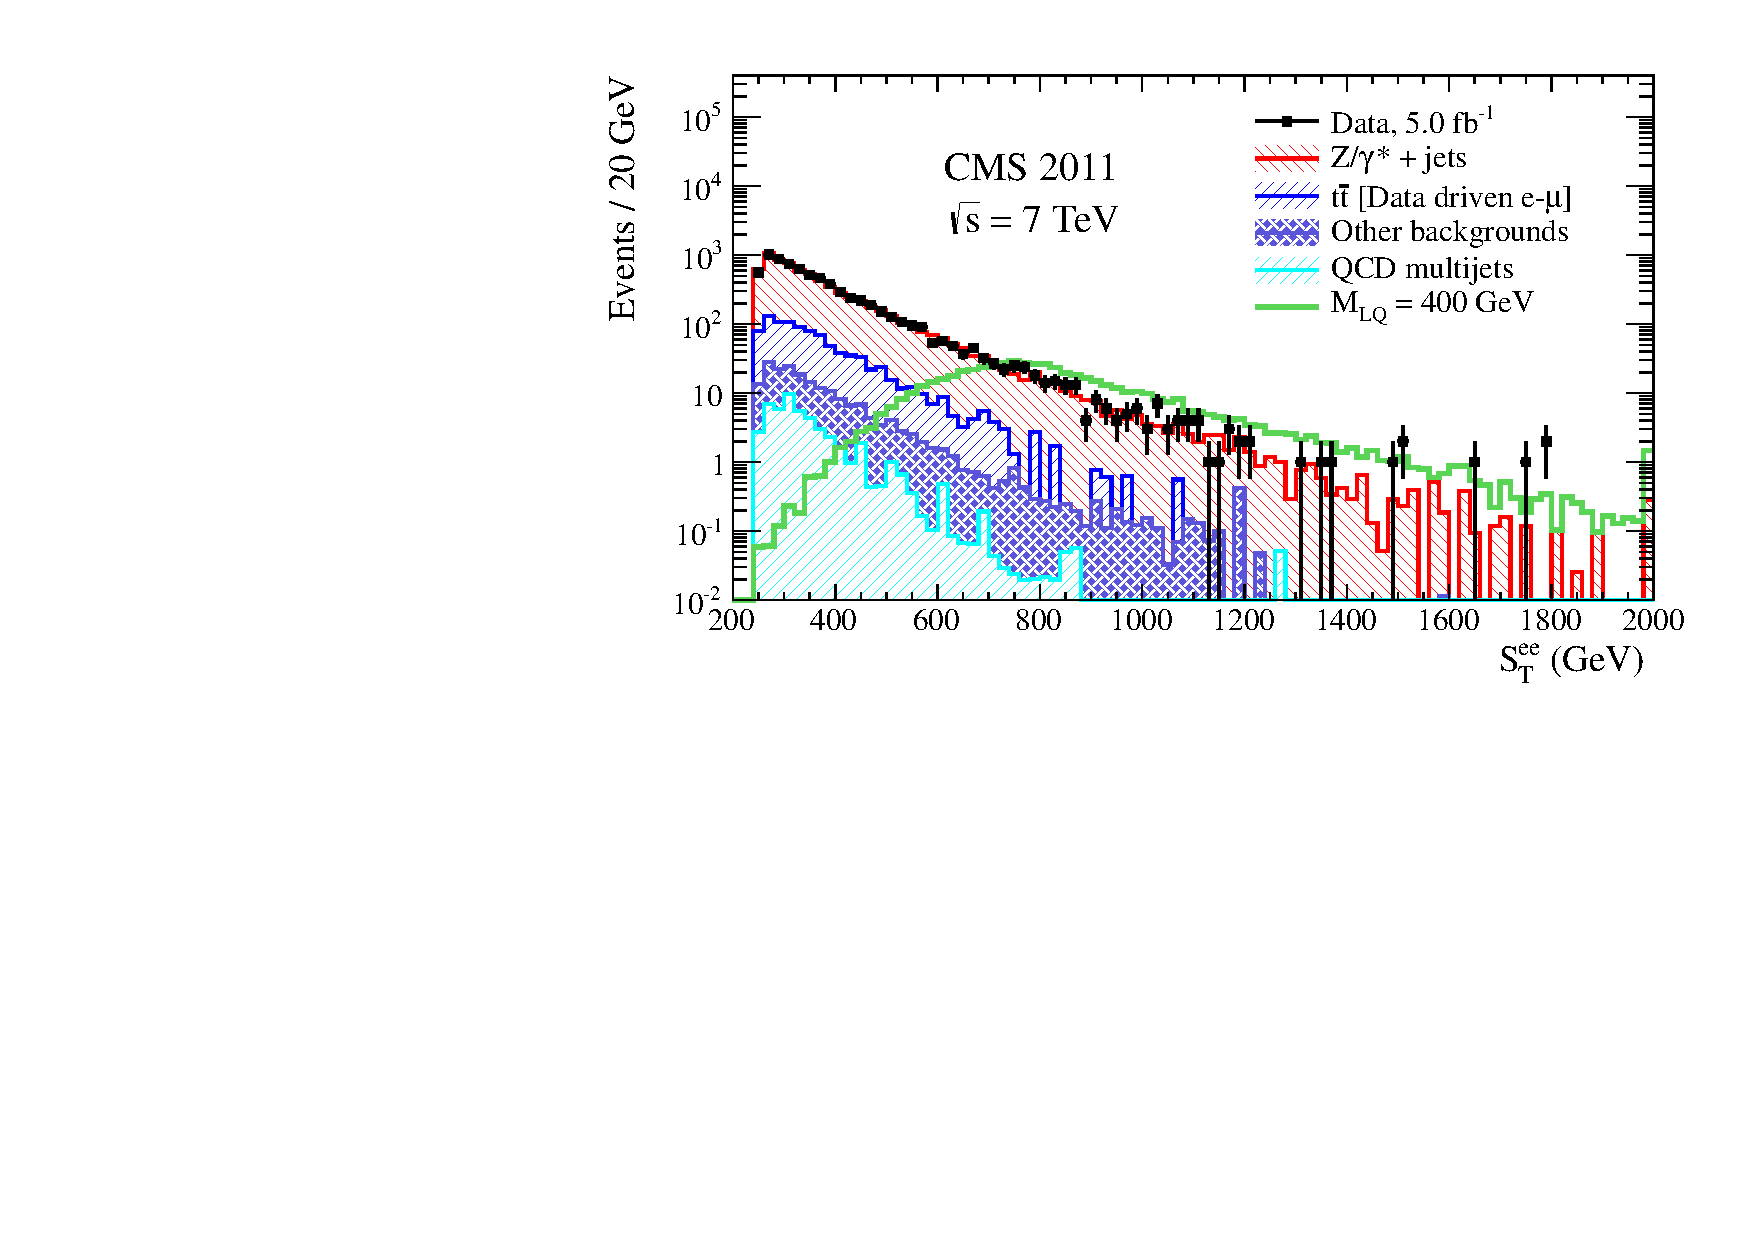
\includegraphics[width=.49\textwidth]{tex/analysis/event_selection/fig/ee/preselection/sT_PAS_eejj_WZSherpa_noNSigma.pdf}}
    {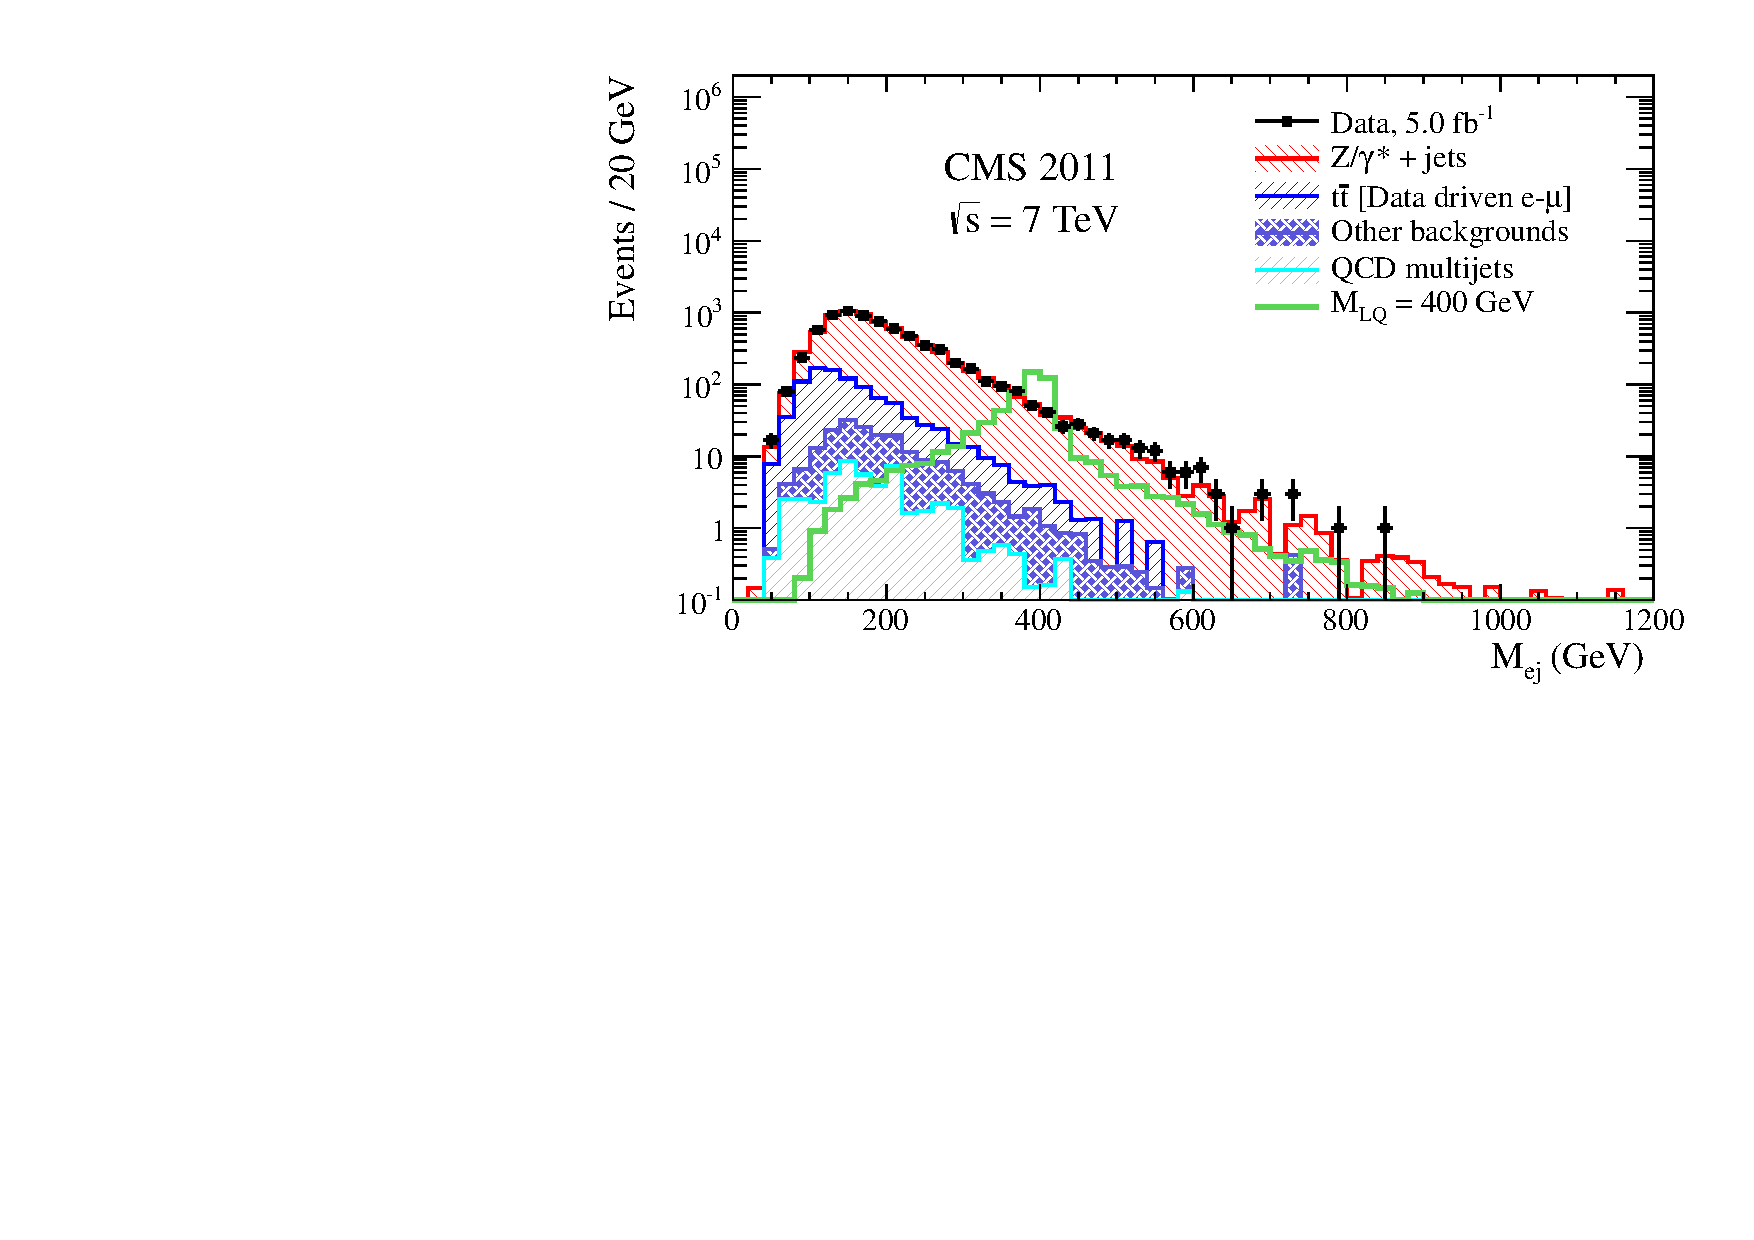
\includegraphics[width=.49\textwidth]{tex/analysis/event_selection/fig/ee/preselection/Mej_selected_avg_PAS_eejj_WZSherpa_noNSigma.pdf}}
    \caption{
      The \st~(left) and \mej~(right) distributions for events
      passing the \eejj~preselection.
    }
    \label{fig:eejj_preselection_st_and_mej}
  \end{center}
\end{figure*}
